\documentclass[20pt,a1paper,portrait,margin=2mm, innermargin=18mm, blockverticalspace=15mm, colspace=15mm, subcolspace=8mm]{tikzposter} 

%\documentclass[20pt,a1paper,landscape,margin=2mm, innermargin=18mm, blockverticalspace=15mm, colspace=15mm, subcolspace=8mm]{tikzposter}

%\documentclass[25pt,a0paper,portrait,margin=2mm, innermargin=28mm, blockverticalspace=20mm, colspace=20mm, subcolspace=10mm]{tikzposter}

%\documentclass[25pt,a0paper,landscape,margin=2mm, innermargin=28mm, blockverticalspace=20mm, colspace=20mm, subcolspace=10mm]{tikzposter}

\usepackage{aigpostersettings}

\usepackage[utf8]{inputenc}
%\usepackage{cite}
\usepackage{pifont}
\usepackage{xcolor}
\usepackage{graphicx}
\usepackage{tikz}
\usetikzlibrary{arrows,automata,positioning,calc,shapes,snakes}

\usepackage{amssymb,amsthm,amsmath}

\usetitlestyle{aigpostertitle1}
%%%%%%%%%%%%%%%%%%%%%%%%%%%%%%%%%%%%%%%%%%%%%%%

\title{\parbox{0.9\linewidth}{\centering Adapted Style after carefully \\ assessing posters during RATIO}}
\institute{Artificial Intelligence Group, University of Hagen} 
\author{Lydia Bl\"umel}


%%%%%%%%%%%%%%%%%%%%%%%%%%%%%%%%%%%%%%%%%%%%%%%%%%%%%%%%%%%%%%



%Titlemaking



%Style-Inclusion from aigpostersettings.sty (check out title options for multiple logos)


\usecolorstyle{aigpostercolor}
\usebackgroundstyle{aigposterback}
\useblockstyle{aigposterblockB}




\begin{document}
	
\maketitle % See Section 4.1
	
	
	
%	\block{Abstract}{Blocktext} % See Section 4.2
	
	\begin{columns}
	\column{0.35}
	
	\block{Example Block A}{
	
		
		\begin{tikzfigure}[A tikz-picture of an AF]
			\label{Fig1:Figure 1}
			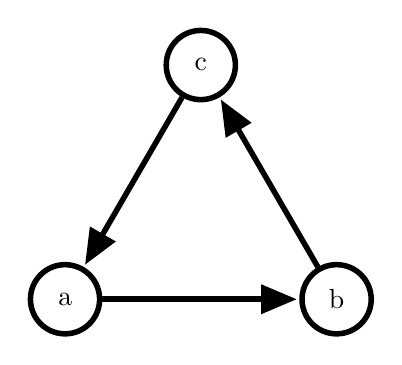
\begin{tikzpicture}[->,>=triangle 45,shorten >=1pt,auto,
				thick]
				\pgfsetlinewidth{2pt}
				\tikzstyle{every state}=[fill=white,draw=black,text=black]
				\node[state]   (A) {a};
				\node[state]   (B) [right = 2.5cm of A]  {b};
				\node[state]   (C) [above = 2.5cm of {$(A)!0.5!(B)$}] {c};
				
				\path (A) edge node {} (B)
				(C) edge node {} (A)
				(B) edge node {} (C);
			\end{tikzpicture}
		\end{tikzfigure}
}
	
	\column{0.65}
	
	\block{Example Block B}{
		Normal text.\vspace{5pt}
		
		
		\begin{itemize}
			\item an item
		\end{itemize}
	    
	    \begin{description}
	    	\item[item] description
	    \end{description}
    
        \begin{enumerate}
        	\item an enumerated item
        \end{enumerate}
	}
	\end{columns}
	
\useblockstyleaigposterblockY	%need special macro for changing the title-color, sry


	\begin{columns} % See Section 4.4
		\column{0.6} % See Section 4.4
		

		\block{Example Block C}{ 
			An equation
			\begin{equation} 
			     \Delta{esign}\quad \Longleftrightarrow\quad \bigcup_{ti}{lity}\ \cup\ Aesthetics  
			\end{equation} 	
		
		
		A table\vspace{5pt}
	   \begin{center}	
		\begingroup
		\renewcommand{\arraystretch}{1.7}
		
		\begin{tabular}{c|c}
			 \textbf{Column 1}  & \textbf{Column 2}	\\ \hline
			 Entry 1 & Entry 2
		\end{tabular}
	\endgroup
	\end{center}
	\vspace{5pt}
	   
       A table as an \yellowhighlight{inner block}\\
       
       \innerblock{\centering
       	\begin{tabular}{c | c}
       		\textbf{Column 1}  & \textbf{Column 2}	\\ \hline
       		Entry 1 & Entry 2 \\
       	\end{tabular}
       } 
   } 

	
 



		
\column{0.4}
		
		


\block{Block D}{
	For discussing "fancy" stuff formats like
\begin{itemize}	
	\item[\ding{228}] cooler itemize versions
\end{itemize}

Btw imho varying block styles help with readability and make things look less monochrome=boring,
use as u see fit
}

\useblockstyleaigposterblockB

\block{TODO}{
	
	\begin{itemize}	
		\item edit blockstyle (requests?)
		\item fix blockstylecommand for style switch
		\item edit highlight-options
		\item \yellowhighlight{add working referencing solution}
		\item add examples for manipulating positioning 
		\item fix multiple logo solutions and title format choice
		\item edit title text format (more bf for title, textwidth)
		\item color itemize symbols
	\end{itemize}
}

%Contact block, may want to include references or a QR-Code for building or?
\block[roundedcorners=5]{}{
\textbf{Contact me} lydia.bluemel@fernuni-hagen.de\\
   or via Teams
}

\end{columns}

\end{document}